\documentclass{article}
% Extra packages for graphics, header control, good math typesetting, and margin
% control:
\usepackage{graphicx, fancyhdr, amssymb, amsmath, geometry}
\geometry{ left = 1.25in, right = 1.25in, top = 1.25in, bottom = 1.25in }
\pagestyle{fancy}
\setlength{\headsep}{.5in}
\renewcommand{\headrulewidth}{.25pt}
\lhead{\footnotesize BLG 454E Learning From Data}
\chead{}
\rhead{\footnotesize \today}

\lfoot{}
\cfoot{\footnotesize Page \thepage}
\rfoot{}
% The right way to define math operators, so that they display with the correct
% font and spacing:
\DeclareMathOperator{\Var}{Var}
\DeclareMathOperator{\Cov}{Cov}
\fancyhead[C]{\em Term Project Report}

    \newcommand\independent{\protect\mathpalette{\protect\independenT}{\perp}}
    \def\independenT#1#2{\mathrel{\setbox0\hbox{$#1#2$}%
    \copy0\kern-\wd0\mkern4mu\box0}} 

\begin{document}

\title{%
  \bf BLG 454E Learning From Data (Spring 2018) \\
  \large Homework I}

\author{\bf Kadir Emre Oto \\ 150140032}
\date{\today}
\maketitle


\section{Question 1} 

$P(A) = \dfrac{1}{4}$ (Rains on Saturday) \\

$P(B) = \dfrac{1}{4} \cdot \dfrac{1}{2} + \dfrac{3}{4} \cdot \dfrac{1}{4} = \dfrac{5}{16} $ (Rains on Sunday) \\

$P(A\ |\ B) = \dfrac{P(A, B)}{P(B)} = \dfrac{\dfrac{1}{4} \cdot \dfrac{1}{2}}{\dfrac{5}{16}} = \dfrac{2}{5}$

\section{Question 2} 

If starting point is in \{A\} $\rightarrow \dfrac{1}{7}$ \\

If starting point is in \{B, F\} $\rightarrow \dfrac{2}{7} \cdot (\dfrac{1}{3} + \dfrac{1}{3} \cdot \dfrac{1}{6}) = \dfrac{1}{9} $ \\

If starting point is in \{G\} $\rightarrow \dfrac{1}{7} \cdot (\dfrac{1}{6} + \dfrac{2}{6} \cdot \dfrac{1}{3}) = \dfrac{5}{126} $ \\

If starting point is in \{C, E\} $\rightarrow \dfrac{2}{7} \cdot (\dfrac{1}{3} \cdot \dfrac{1}{6} + \dfrac{1}{3} \cdot \dfrac{1}{3}) = \dfrac{1}{21} $ \\

If starting point is in \{D\} $\rightarrow \dfrac{1}{7} \cdot (\dfrac{1}{3} \cdot \dfrac{1}{6}) = \dfrac{1}{126}$ \\

$Answer = \dfrac{1}{7} + \dfrac{1}{9} + \dfrac{5}{126} + \dfrac{1}{21} + \dfrac{1}{126} = \dfrac{22}{63} $

\section{Question 3} 

$\mu = \dfrac{\Sigma{x_i}}{n},\ \ \sigma^2 = \dfrac{\Sigma{(x_i-\mu})^2}{n}$

$P(x_1, x_2 ... x_n |\ \mu, \sigma^2 ) = \dfrac{1}{\sigma \cdot \sqrt{2\cdot\pi}} \cdot e^{\dfrac{-(x-\mu)^2}{2*\sigma^2}}$


\begin{figure}
  \centering
  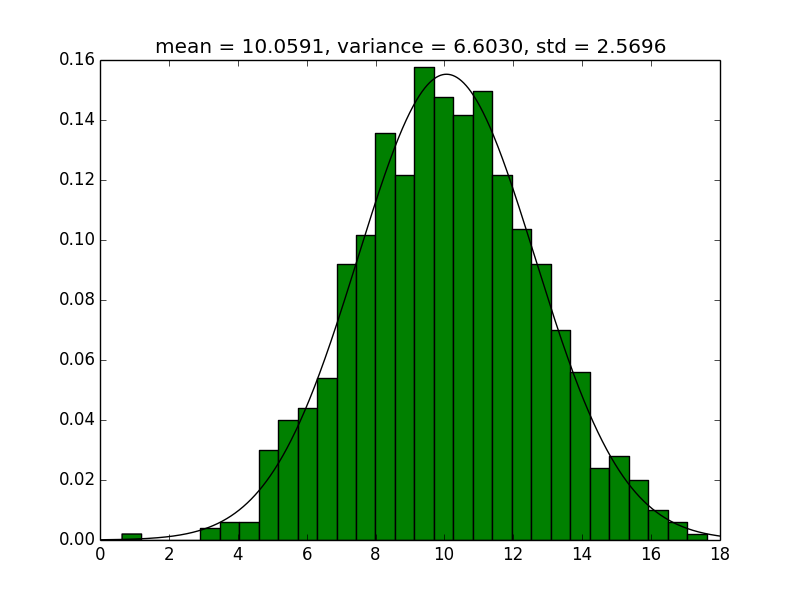
\includegraphics[width=0.8\linewidth]{figure_1.png}
  \caption{A Data and fixed gaussian distribution with MLE}
  \label{fig:figure1}
\end{figure}

\newpage
\section{Question 3} 

\ a) Naive Bayes classifier:
\begin{center}
    \begin{tabular}{ | c | c  c | c c | c c |}
    \hline
     & $X_1$ & & $X_2$ & & $X_3$ & \\ \hline
    Likelihood & YES & NO & YES & NO & YES & NO \\ \hline
    + & $\dfrac{3}{5}$ & $\dfrac{2}{5}$ & $\dfrac{2}{5}$ & $\dfrac{3}{5}$ & $\dfrac{4}{5}$ & $\dfrac{1}{5}$ \\[20pt] \hline
    - & $\dfrac{2}{5}$ & $\dfrac{3}{5}$ & $\dfrac{2}{5}$ & $\dfrac{3}{5}$ & $\dfrac{1}{5}$ & $\dfrac{4}{5}$ \\[20pt] \hline
    \end{tabular}
\end{center}

\ b) 

\ \ \ \ probability that the given data is +: \\


{\centering

  $P(+\ | \ x_1 \cap x_2 \cap x_3) = \dfrac{P(x_1\ | \ +) \cdot P(x_2\ | \ +) \cdot P(x_3\ | \ +) \cdot P(+)}{P(x_1) \cdot P(x_2) \cdot P(x_3)}$ \\ 

  $ = \dfrac{3}{5} \cdot \dfrac{2}{5} \cdot \dfrac{4}{5} \cdot \dfrac{1}{2} = \dfrac{12}{125} $\par
}

\ \ \ \ probability that the given data is -: \\

{\centering

  $P(-\ | \ x_1 \cap x_2 \cap x_3) = \dfrac{P(x_1\ | \ -) \cdot P(x_2\ | \ -) \cdot P(x_3\ | \ -) \cdot P(-)}{P(x_1) \cdot P(x_2) \cdot P(x_3)}$ \\ 

  $ = \dfrac{2}{5} \cdot \dfrac{2}{5} \cdot \dfrac{1}{5} \cdot \dfrac{1}{2} = \dfrac{2}{
  125}$ \\

  $\dfrac{P(+\ | \ x_1 \cap x_2 \cap x_3)}{P(+\ | \ x_1 \cap x_2 \cap x_3) + P(-\ | \ x_1 \cap x_2 \cap x_3)} = \dfrac{6}{7}$ \par
}


\ c) 

{\centering
	$P(x_1) = \dfrac{1}{2}$ \\
	$P(x_2) = \dfrac{2}{5}$ \\
	$P(x_1\ | \ x_2) = \dfrac{1}{2}$ \\
	$P(x_1, x_2) = \dfrac{1}{5}$ \\

	$P(x_1, x_2) = P(x_1\ | \ x_2) \cdot P(x_2) = \dfrac{1}{2} \cdot \dfrac{2}{5} = \dfrac{1}{5}$

	Because of the formulas above give the same result, we can say $x_1$ and $x_2$ are dependent.
	\par
}


\end{document}
